% =====================================================================
% Chapter: Laplace Approximation: Null Space Posterior
% (pass for narrative coherence + notation consistency vs previous Laplace chapter)
% =====================================================================

% --- Local helpers (keep lightweight; use \providecommand to avoid redefinition errors) ---
\providecommand{\R}{\mathbb{R}}

\newenvironment{smallpmatrix}
  {\left(\begin{smallmatrix}}
  {\end{smallmatrix}\right)}

\renewcommand{\paragraph}[1]{\textbf{#1}~~} % a more space-efficient layout

% Fallback if pifont isn't loaded (so compilation doesn't hard-fail)
\providecommand{\ding}[1]{\ensuremath{\checkmark}}
\providecommand{\cmark}{\ding{51}}%
\providecommand{\xmark}{\ding{55}}%

% If your preamble doesn't define \smaller[<scale>]{...}, provide a scale-factor version.
\providecommand{\smaller}[2][0.9]{\scalebox{#1}{#2}}

% Core notation aligned with Chapter~\ref{ch:laplace} (use plain \theta, \theta_{\textsc{map}}, \mathrm{GGN}, etc.)
\providecommand{\J}{\mathbf{J}}      % Jacobian
\providecommand{\U}{\mathbf{U}}      % Matrix U
\providecommand{\mat}[1]{\mathbf{#1}}
\providecommand{\vec}[1]{\mathbf{#1}}
\providecommand{\x}{\mathbf{x}}
\providecommand{\y}{\mathbf{y}}
\providecommand{\N}{\mathcal{N}}
\providecommand{\T}{^{\top}}
\providecommand\norm[1]{\left\lVert#1\right\rVert}
\providecommand{\trace}{\mathrm{Tr}}
\providecommand{\MAP}{\textnormal{\textsc{map}}}
\providecommand{\GGN}{\mathrm{GGN}}
\providecommand{\LLA}{\textsc{lla}}

\providecommand{\marco}[1]{{\textcolor{purple}{Marco: {#1}} }}
\providecommand{\hrittik}[1]{{\textcolor{blue}{Hrittik: {#1}} }}
\providecommand{\hauberg}[1]{{\textcolor{red}{[Søren says: {#1}]} }}
\providecommand{\first}[1]{\textbf{#1}}

\definecolor{myblue}{RGB}{218, 232, 252}

\frenchspacing
\hyphenation{de-com-posi-tion}

\chapter{Laplace Approximation: Null Space Posterior}
\label{ch:laplace_null}

\begin{keypointsbox}
\textbf{Key points (Chapter~\thechapter).}
\begin{enumerate}
    \item \textbf{Linearised Laplace without underfitting.}
    Building on the theoretical analysis of Laplace Approximations from \cref{ch:laplace}, we develop and approximation of Linearised Laplace that is optimal for noiseless data and shows no underfitting. We call it the \emph{Projected Posterior}.
    \item \textbf{Scalability.} We develop a memory-efficient sampling algorithm that can sample from the parameter space of arbitrarily large models at the cost of a few epochs of training.
\end{enumerate}
\end{keypointsbox}

\begin{center}
\begin{minipage}{0.95\linewidth}
\noindent\textbf{Chapter \thechapter\ -- Laplace Approximation: Null Space Posterior}\par\vspace{3pt}

\begin{tabular}{@{}p{0.83\linewidth}r@{}}
\hyperref[sec:underfitting]{\thechapter.1\;\;Underfitting in Bayesian deep learning} \dotfill & \pageref{sec:underfitting}\\

\hyperref[sec:nullspace_posterior]{\thechapter.2\;\;Null-Space Posterior} \dotfill & \pageref{sec:nullspace_posterior}\\
\hyperref[sec:null_results]{\thechapter.3\;\;Experiments} \dotfill & \pageref{sec:null_results}\\
\end{tabular}
\end{minipage}
\end{center}

So far we have studied the geometry of the parameter space in Bayesian deep learning in \cref{chap:setting} and practical algorithms for making computations in the parameter space equipped with this geometry in \cref{chap:linalg}. In Chapter~\ref{ch:laplace}, we used this geometric viewpoint to understand the uncertainties arising from Laplace approximations and, more generally, to shed light on some of the problems encountered in Bayesian deep learning. More specifically, decomposing the uncertainty into its two fundamental components and how they interact with the choice of the predictive (neural network or the linearized neural network). The Laplace diffusion proposed in \Cref{ch:laplace}, is meant to be a simple modification of Laplace approximation as close as possible to the theoretical ideal. In other words, the focus there was on theory-validation rather than the usual focus on performance and scalability. However, this raises an obvious question: can we build on the theoretical insights to build practical, performant, and scalable Bayesian Methods? In this chapter, this is precisely the question we will attempt to answer. 

Building on the understanding of why Linearised Laplace works well, from \Cref{ch:laplace}, we will build an approximation that preserves the training predictions of the \textrm{MAP} estimate. We propose to build Bayesian approximations in the Jacobian null space, thereby guaranteeing that the Bayesian predictive does not underfit. An extensive empirical evaluation shows that the approach scales to large models, including vision transformers with 28 million parameters.


\section{Underfitting in Bayesian deep learning}
\label{sec:underfitting}
Bayesian deep learning tends to underfit. \cref{ch:laplace} demonstrates that marginalizing approximate weight posteriors from Laplace Approximation yields less accurate predictions than applying a \emph{maximum a posteriori} (\textsc{map}) point estimate. This significantly reduces the practical value of Bayesian deep learning, despite having attractive theoretical properties \citep{germain2016pac}.
%
As we also saw in \cref{ch:laplace}, Linearised Laplace does not suffer from the underfitting issue. And further, this is primarily because its kernel component does not add variance in-distribution, causing its predictive variance to be low in-distribution and high out-of-distribution. We will build on this observation.
We first explicate \emph{why} underfitting happens with Gaussian approximate posteriors, and thereafter propose a solution for low-noise data (e.g.\@ images).



\begin{figure}
  %\vspace{-5mm}
  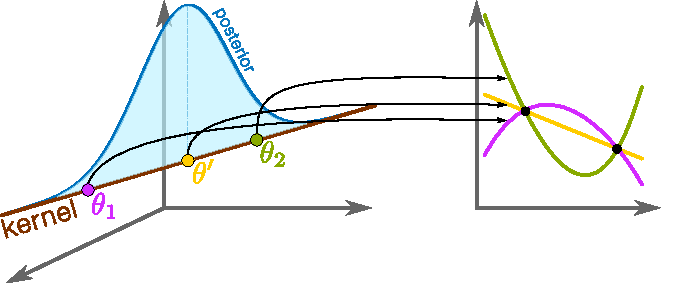
\includegraphics[width=\linewidth]{chapters/ch6_figures/idea.pdf}
  \vspace{-7mm}
  \caption{\emph{Key idea:} In overparametrized linear models, the \emph{kernel} (null space) contains all models that have identical predictions on the training data. We propose restricting approximate posteriors of deep neural networks to this kernel to avoid underfitting.}
  \label{fig:idea}
\end{figure}
%
\paragraph{What is underfitting?}
Deep learning performs very well when the training data is subject to limited observation noise. In contrast, Bayesian deep learning often \emph{underfits} in the sense that the Bayesian prediction deviates significantly from a \emph{point estimate} prediction \emph{on the training data} $\mathcal{D}$, i.e.
\begin{align}
  %\hspace{-2cm}\text{Bayesian underfitting:}\qquad\qquad
  \mathbb{E}_{\theta \sim q} \left[f(\theta, \x)\right] \neq f(\theta_{\textsc{map}}, \x)
  \qquad
  \text{for } \x \in \mathcal{D},
\end{align}
%
where $q$ is an approximate posterior and $\theta_{\textsc{map}}$ is a point estimate of the neural network $f$.
This notion of underfitting only applies to low-noise data, where the posterior should have little uncertainty on the training data, but this is the most prominent scenario in deep learning. \looseness=-1 %In this case, samples from the posterior will interpolate the training data. % (Fig.~\ref{fig:interpolation}).


\textbf{Why do Bayesian neural networks underfit?}
Deep neural networks are commonly \emph{overparametrized}, i.e.\@ the model has more parameters than observations, as this tends to improve both optimization and generalization \citep{allen2019learning}. Fig.~\ref{fig:idea} sketches the situation which we later formalize: Consider fitting a quadratic function with three parameters to only two observations. This leaves one degree of freedom undetermined and a linear subspace of the model parameters exists wherein all parameters yield identical predictions on the training data. For low-noise data, the true posterior will concentrate around this subspace. Unfortunately, common Gaussian approximations to the posterior are axis-aligned (i.e.\@ \emph{mean field} approximations \citep{bishop2006pattern}) and not aligned with the mentioned subspace. This mismatch leads to a poor posterior approximation that tends to underfit. \emph{We suggest, quite simply, to project the approximate posterior to the subspace in which underfitting cannot happen.}
% However, practical Bayesian approximations, such as variational inference \citep{xxx}, are not designed with overparameterization in mind. 

\paragraph{Why is this beneficial?}
%Being Bayesian brings benefits, such as reliable out-of-distribution detection and general uncertainty quantification. 
Our proposed posterior reflects the degrees of freedom in the model that fundamentally cannot be determined by even noise-free data. Predicting according to this distribution gives reliable out-of-distribution detection and general uncertainty quantification without underfitting. 
Our approach captures correlations between layers and retains high-accuracy predictions while scaling linearly with model size. %Elegantly, our approach works for any differentiable model, unlike e.g.\@ \textsc{kfac} \citep{dangel2020backpack} which requires network-specific implementations. Our open-source implementation is applicable whenever we can access Jacobian-vector and vector-Jacobian products. 
Table~\ref{tab:models} contrasts our method with existing ones.\looseness=-1

\paragraph{Why is this difficult?}
We will soon see that the relevant subspace on which to project is given by the \emph{kernel} (i.e.\@ \emph{null space}) of a matrix that is quadratic in the number of model parameters. Even for models of modest size, this matrix is too large to be stored in memory and direct projection methods cannot be applied. \emph{We propose a linear-time sampling algorithm that can be implemented entirely using automatic differentiation.}


% \hrittik{Some more benefits we can list here:
% \begin{enumerate}
%     \item Out method is model agnostic. Many approximate bayesian inference methods, such as KFAC, require specific implementation for different layers. Projection algorithm, by contrast, can be applied to any model as long as we have access to efficient Jacobian Vector Products and Vector Jacobian products of the model and its loss. 
%     \item While in this work we apply the projection algorithm to Laplace approximation, the projection can be applied in a post-hoc manner to any approximate bayesian method which relies on monte-carlo sampling from the posterior to make predictions. If the bayesian method suffers from underfitting the projection will alleviate this issue.
% \end{enumerate}}
%\hauberg{Write about the benefits of our approach and reference table~\ref{tab:models}.}
%Captures correlation between layers without a quadratic scaling in number of parameters.
%Retains high-accuracy predictions while allowing for useful uncertainty quantification.
%Scales to large models.

\begin{table*}[t]
	\vspace*{-1.0\baselineskip}
	\centering
        \begin{center}
	\caption{Comparisons between Laplace approximations. $N$: number of data points, $O$: output dimensions, $P$: number of parameters, $P_{l,in}$, $P_{l,out}$: input and output dimensions of layer $l$, $P_{ll}$: last layer parameters.} 
 \vspace{-3mm}
 % \marco{Isn't Diagonal also model agnostic?}}
 %    \hrittik{Yes in a way you are right. Out jax implementation of both last layer and diagonal are model-agnostic but in Laplace redux and specifically backpack it is not. They write custom derivatives for all the layers: \href{https://github.com/f-dangel/backpack/tree/master/backpack/extensions/secondorder/diag_ggn}{backpack}. So yeah not sure how to write that in the table maybe a (?)}
 %    \marco{But that's only a PyTorch limitation, not a method limitation. I think it is more fair to write \cmark in the table}
    \label{tab:models}
	\resizebox{1.0\textwidth}{!}{%
		\begin{tabular}{cccccccc}
			\toprule
			%\textsc{Method} & \textsc{Correlation Structure} & \textsc{Space Complexity} & \textsc{Time Complexity} & \textsc{Error Bound} & \textsc{Model Agnostic} & \textsc{Tractable LML}\\
			\textsc{Method} & \textsc{Correlation} & \textsc{Space}      & \textsc{per-sample Time}       & \textsc{preprocessing Time}      & \textsc{Error} & \textsc{Model}    & \textsc{Tractable} \\
                            & \textsc{structure}   & \textsc{complexity} & \textsc{complexity} & \textsc{complexity} & \textsc{bound} & \textsc{agnostic} & optimal \textsc{lml} \\
            %
			\midrule
			Diagonal & 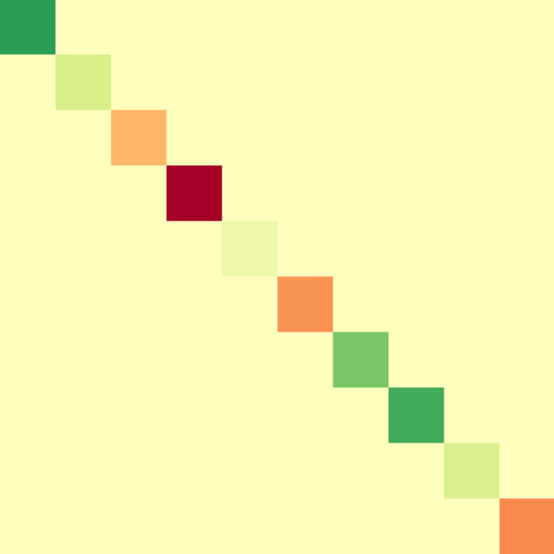
\includegraphics[width=0.07\linewidth]{chapters/ch6_figures/diag2.pdf} & $P$ & P & $PNO$ & \xmark & \cmark & \xmark \\
			Kronecker-Factored & 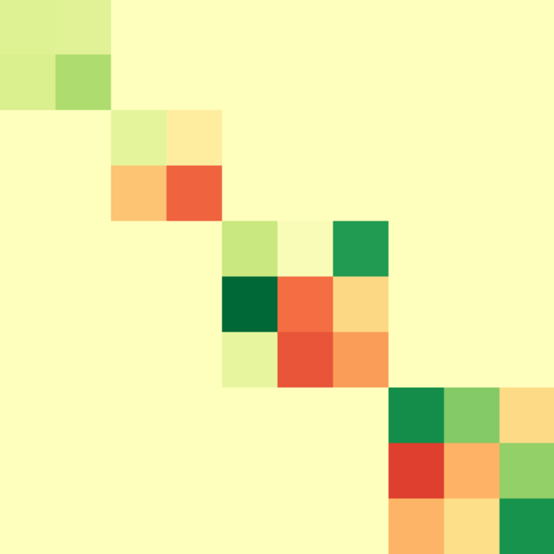
\includegraphics[width=0.07\linewidth]{chapters/ch6_figures/kfac2.pdf} & $\sum_{l=1}^L P_{l,in}^2 + P_{l,out}^2$  & $\sum_{l=1}^L P_{l,in}^2 \!+\! P_{l,out}^2$ & $\sum_{l=1}^L \! NP_{l,in} \!+\! NP_{l,out} \!+\! P_{l,in}^3 \!+\! P_{l,out}^3$ 
   & \xmark & \xmark & \xmark\\
   			Last-Layer & 
\includegraphics[width=0.07\linewidth]{chapters/ch6_figures/ll_diag2.pdf} & $P_{ll}^2$ & $P_{ll}^2$ & $O^2N P_{ll}^2 + P_{ll}^3$ & \xmark & \cmark & \xmark\\
%			\textbf{Projected posterior (Ours)} & 
\includegraphics[width=0.03\linewidth]{figures/proj2.pdf} & $P+NO^2$ & $t_{\max}PN+NO^3$ & 0 & \cmark~(Lemma.~\ref{lm:error_bound})  & \cmark & \cmark~(Sec.~\ref{sec:3.3})\\
%			\textbf{Loss-Projected posterior (Ours)} & 
\includegraphics[width=0.03\linewidth]{figures/proj2.pdf} & $P+N$ & $t_{\max}PN$ & 0 & \xmark  & \cmark & \xmark \\
			Projected Posterior %($q_{\textnormal{\textsc{proj}}}$ or $q_{\textnormal{\textsc{loss}}}$)  %what do you think about this?
            & 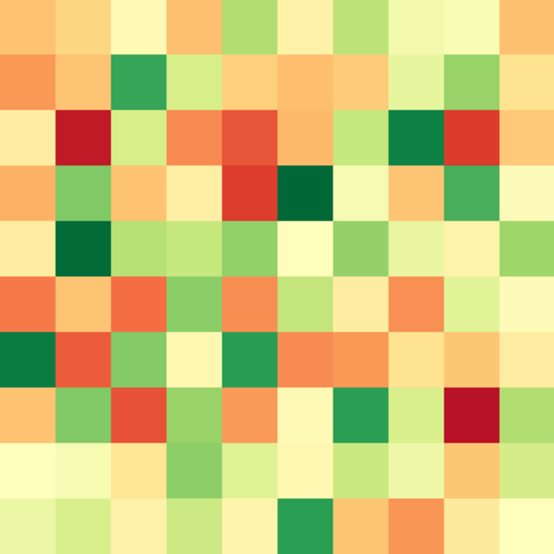
\includegraphics[width=0.07\linewidth]{chapters/ch6_figures/proj2.pdf} & $P+NO^2$ or $P+N$ & $t_{\max}PN+NO^3$ or $t_{\max}PN$ & 0 & \cmark~(Lemmas~\ref{lm:error_bound} \& \ref{lm:loss_proj_err})  & \cmark & \cmark~(Sec.~\ref{sec:null:model_selection}) \\
			\bottomrule
	\end{tabular}}
        \end{center}	
	\vspace*{-0.5\baselineskip}
\end{table*}


\section{Null-Space Posterior}
\label{sec:nullspace_posterior}
We next propose a fully correlated Gaussian posterior that is guaranteed to not underfit (for the linearised model).

As alluded to, we propose restricting the posterior covariance to a particular subspace of the parameter space. Letting $\U \in \R^{P \times R}$ denote an orthogonal basis of this subspace, we consider an \emph{isotropic} model therein,
\begin{equation}
    q_{\textnormal{\textsc{proj}}}(\theta \mid \theta_{\textsc{map}}, \mathcal{D})
    =
    \mathcal{N}\!\left(\theta \mid \theta_{\textsc{map}},\ \alpha^{-1}\U\U\T \right).
    \label{eq:null:approx_post}
\end{equation}
Specifically, we choose the above subspace as the \emph{kernel} (i.e.\@ \emph{null space}) of the $\GGN$\ matrix at the mode and call the result the \emph{projected posterior}. This is precisely the kernel component of linearised Laplace in \cref{fig:laplace_decomp}. Formally,
\begin{align}
  \U\U\T
  =
  \mathbb{I}_P - \mathcal{P}(\GGN)
  =
  \mathbb{I}_P - \mat{V}\, [\mat{D} \!>\! 0]\, \mat{V}\T,
  \label{eq:null:proj_def}
\end{align}
where $\mat{V}\mat{D}\mat{V}\T$ is an eigen decomposition of $\GGN_{\theta_{\textsc{map}}}$ and $[\mat{D} \!>\! 0] \in \R^{P \times P}$ is diagonal with elements 1 where $\mat{D}$ holds positive values. We use the shorthand $\mathcal{P}(\GGN)$ to denote the projection onto the image of the $\GGN$.

\emph{We next justify the projected posterior through the lens of underfitting.}

\paragraph{The projected posterior never underfits (for the linearised model).}
When using the linearised neural network,
\begin{align}
f_{\mathrm{lin}}^{\theta_{\textsc{map}}}(\theta, x)
=
f(\theta_{\textsc{map}}, x) + \J_{x}(\theta_{\textsc{map}})\,(\theta-\theta_{\textsc{map}}), 
\end{align}
we avoid underfitting on the training data when $\J_{x}(\theta_{\textsc{map}})(\theta-\theta_{\textsc{map}}) = \mathbf{0}$ for all $\x\in\mathcal D$. The linearised model thus avoids underfitting when $\theta-\theta_{\textsc{map}}$ is restricted to the kernel of the stacked dataset Jacobian
\begin{align}
    \J_{\mathcal D}(\theta_{\textsc{map}})
=
\begin{pmatrix}
\J_{x_1}(\theta_{\textsc{map}})\\ \vdots \\ \J_{x_N}(\theta_{\textsc{map}})
\end{pmatrix}\in\R^{NO\times P}.
\end{align}
For the proposed projected posterior \eqref{eq:null:approx_post}, we choose $\U$ as an orthonormal basis of this Jacobian kernel and note that this kernel coincides with the zero-eigenspace of $\GGN_{\theta_{\textsc{map}}}$. \looseness=-1

These considerations can be formalised as follows.
\begin{lemma}
\label{lm:null:zero_var_train}
    The projected posterior \eqref{eq:null:approx_post} is supported on equal functions on the training data, i.e.\@ for all $\x \in \mathcal{D}$,
    \begin{align}
        f_{\mathrm{lin}}^{\theta_{\textsc{map}}}(\theta, x) = f(\theta_{\textsc{map}}, x)
        \qquad
        \forall \theta \sim q_{\textnormal{\textsc{proj}}},
    \end{align}
    which implies that~~$\textnormal{\textsc{Var}}_{\theta \sim q_{\textnormal{\textsc{proj}}}} f_{\mathrm{lin}}^{\theta_{\textsc{map}}}(\theta, x) = 0$.
\end{lemma}
We emphasize that the statement \emph{only holds on the training data}. Elsewhere, the approximate posterior yields strictly positive variances with high probability under strong but reasonable assumptions.

\begin{restatable}{lemma}{PositiveVarianceLemma}
  \label{lm:null:variance_nonzero_test}
    Let $x_{\textnormal{test}} \in \R^I$. Then
    \begin{equation}
    \label{eq:null:variance_nonzero_test}
        \textnormal{\textsc{Var}}_{\theta \sim q_{\textnormal{\textsc{proj}}}} f_{\mathrm{lin}}^{\theta_{\textsc{map}}}(\theta, x_{\textnormal{test}}) > 0
    \end{equation}
    if
    \resizebox{0.95\linewidth}{!}{$\textnormal{\textsc{Rank}}\!\left(\begin{smallpmatrix}
        \J_{\mathcal D}(\theta_{\textsc{map}}) \\ \J_{x_{\textnormal{test}}}(\theta_{\textsc{map}})
    \end{smallpmatrix}\!
    \begin{smallpmatrix}
        \J_{\mathcal D}(\theta_{\textsc{map}}) \\ \J_{x_{\textnormal{test}}}(\theta_{\textsc{map}})
    \end{smallpmatrix}\!\T\right)
    >
    \textnormal{\textsc{Rank}}\left(\J_{\mathcal D}(\theta_{\textsc{map}})\, \J_{\mathcal D}(\theta_{\textsc{map}})\T\right)$.}
\end{restatable}

Jointly, Lemma~\ref{lm:null:zero_var_train} and Lemma~\ref{lm:null:variance_nonzero_test} show that out-of-distribution data is guaranteed to have higher predictive variance than the training data. The (technical) rank assumption in Lemma~\ref{lm:null:variance_nonzero_test} is known to be satisfied with high probability under reasonable assumptions \citep{bombari2022memorization, nguyen2021tight, karhadkar2024bounds}. \looseness=-1

These results can be contrasted with \LLA, where we can show the following result.
\begin{restatable}{theorem}{UpperBoundLinearizedLaplace}
\label{thm:null:upper_bound_lla}
    For $\alpha>0$, the predictive variance of \LLA\ on any training datapoint is positive and bounded,
    \begin{equation*}
        \frac{O \gamma^2}{\gamma^2 + \alpha}
        \leq
        \textnormal{\textsc{Var}}_{\theta\sim q_{\textnormal{\textsc{lla}}}} f_{\mathrm{lin}}^{\theta_{\textsc{map}}}(\theta, x)
        \leq
        \frac{O \lambda^2}{\lambda^2 + \alpha}
        \quad \text{for } x \in \mathcal{D}.
    \end{equation*}
    Here, $\lambda$ and $\gamma$ are the largest and smallest singular values of the dataset Jacobian $\J_{\mathcal D}(\theta_{\textsc{map}})$, respectively.
\end{restatable}
Here, $\gamma$ is strictly positive with high probability under reasonable assumption \citep{bombari2022memorization, nguyen2021tight, karhadkar2024bounds}. \emph{\LLA\ then underfits with high probability, which contrasts our approach (c.f.\@ Lemma~\ref{lm:null:zero_var_train})}.
Note that this is only true for the (intractable) $\GGN$-based covariance. We expect that sparse approximations to this covariance, e.g.\@ diagonal and \textsc{kfac}, have even higher training-set variance.

\paragraph{Underfitting in existing models.}
The above analysis justifies the projected posterior and also sheds light on why current Bayesian approximations often underfit. For efficiency, mean-field approximations of the posterior covariance are quite common, e.g.\@ \emph{diagonal} or \emph{Kronecker factored} covariances \citep{ritter2018scalable, martens2015optimizing}. These approximations will generally sample outside the $\GGN$ kernel, implying strictly positive predictive variances on the training data even for noise-free data. This reasoning also motivates recent works that have attempted to improve these approximations by making their spectrum more aligned with the spectrum of the $\GGN$ \citep{george2018fast, dhahri2024shaving}.

\paragraph{Computational benefits.}
Beyond the above theoretical motivations, our projected covariance also brings computational benefits. Since $\U$ is an orthonormal basis, the covariance $\U\U\T$ is a projection matrix, implying that its eigenvalues are all 0 or 1. This, in turn, implies that $\U\U\T = (\U\U\T)^2 = (\U\U\T)\T = (\U\U\T)^{\dagger}$, where $^{\dagger}$ denotes pseudo-inversion. Drawing samples from $q_{\textnormal{\textsc{proj}}}$ thus only requires matrix-vector products with $\U\U\T$ and the matrix need not be instantiated.
The only open question is then how to perform such matrix-vector products efficiently; this is addressed by the projection primitives from Chapter~\ref{chap:linalg}. \looseness=-1

Since all eigenvalues of $\U\U\T$ are 0 or 1, we can a priori expect the matrix to yield numerically stable computations even at moderate numerical precision. This is in contrast to the $\GGN$, which easily has condition numbers that exceed $10^6$ \citep{miani:sketching:2024}.


\paragraph{Tractable model selection.}
\label{sec:null:model_selection}
A benefit of Bayesian neural networks is that we can choose $\alpha$ by maximising the marginal likelihood, $p(\mathcal{D}\mid\alpha)$, on the training data, i.e.\@ without relying on validation data \citep{mackay1995probable}. However, since the marginal likelihood of the true posterior is intractable, it is common to consider that of the Laplace approximation \citep{immer2021scalable}
\begin{align}
\label{eq:null:lml}
\begin{split}
    \log \, q_{\textsc{lla}}(\mathcal{D}\mid\alpha)
      &=
      \log\,p(\mathcal{D}\mid \theta_{\textsc{map}}) + \log\, p(\theta_{\textsc{map}}\mid\alpha)  \\
      &- \frac{1}{2} \log\det\!\left( \frac{1}{2\pi}\left(\GGN_{\theta_{\textsc{map}}} + \alpha \mathbb{I}\right) \right).
\end{split}
\end{align}
This can then be optimised numerically to estimate $\alpha$. In contrast, the projected posterior \eqref{eq:null:approx_post} does not require optimisation as $\alpha$ is available in closed form.
\begin{lemma}
\label{lm:null:opt_alpha}
    The marginal likelihood for the projected posterior \eqref{eq:null:approx_post} has a globally optimal $\alpha$ given by
    \begin{equation}\label{eq:null:opt_alpha}
        \alpha^* = \frac{\norm{\theta_{\textsc{map}}}^2}{P - \trace\!\big(\mathbb{I}_P - \mathcal{P}(\GGN_{\theta_{\textsc{map}}})\big)}.
    \end{equation}
\end{lemma}
In practice, the trace can be approximated using \citeauthor{hutchinson1989stochastic}'s estimator [\citeyear{hutchinson1989stochastic}].

\paragraph{Links to \LLA.}
The projected posterior can be viewed as a fully correlated tractable approximation to \LLA. The following statement shows that the difference between the two approximate posteriors is bounded.
\begin{lemma}\label{lm:null:error_bound}
   Let $\tau$ denote the smallest non-zero eigenvalue of $\GGN_{\theta_{\textsc{map}}}$ \citep{nguyen2021tight}, then
\begin{equation*}
    \Big\|
    \underbrace{\big(\alpha \mathbb{I}_P + \GGN_{\theta_{\textsc{map}}}\big)^{-1}}_{\textnormal{\LLA\ covariance}}
    -
    \underbrace{\alpha^{-1}\big(\mathbb{I}_P - \mathcal{P}(\GGN_{\theta_{\textsc{map}}})\big)}_{\textnormal{projected covariance (scaled)}}
    \Big\|
    \leq
    \frac{1}{\tau + \alpha}.
\end{equation*}
Additionally, let $k$ denote the rank of $\GGN_{\theta_{\textsc{map}}}$ and let $d$ be the $W_2$ Wasserstein distance, then $d^2(q_{\textnormal{\textsc{lla}}}, q_{\textnormal{\textsc{proj}}}) \leq (\tau + \alpha)^{-1} k$.
\end{lemma}

\subsection{Efficient Sampling from the Projected Posterior}

We next develop a novel scalable algorithm to sample the projected posterior.
Recall that we can simulate this posterior as $\U \U\T \epsilon + \theta_{\MAP}$, where $\epsilon \sim \N(\mathbf{0}, \alpha^{-1}\mathbb{I})$ and $\U\U\T$ projects to the \textsc{ggn} kernel. Following the discussion from \cref{chap:linalg}, we note that instead of working with the $\U\U\T $, which is an intractable $P \times P$, matrix we can work with the linear operator that multiplies any vector with this matrix. This operator is precisely the $ \textsf{Proj}_V$ operator from \cref{sec:subspace_projections}. We have discussed there how to efficeintly apply this operator to arbitrary vector without instantiating any large matrices, giving us an efficient low-memory sampling algorithm.

\paragraph{Complexity.} The space complexity of the algorithm is $\mathcal{O}(P + NSO^2)$ and time complexity is $\mathcal{O}(t_{\max}PN+N S^2 O^3)$. For overparametrized models where $P \gg NO$ these complexities boil down to $\mathcal{O}(P)$ and $\mathcal{O}(t_{\max}PN)$, respectively. This matches the cost of training for $t_{\max}$ epochs.
Consequently, the projection is feasible on hardware that can train a model.


\paragraph{Scaling to high-dimensional outputs}
\label{subsec:null:high_dim_outputs}
The computational complexity of the projection algorithm scales superlinearly with the model's output size. For many tasks this is unproblematic, but it renders the method inapplicable to e.g.\@ image-generative models.

To handle high-dimensional outputs, we propose removing the requirement of preserving the predictions of $\theta_{\textsc{map}}$ on the training data. Instead, we propose to (locally) preserve the \emph{loss} at each training point.
This is achieved by considering the loss-Jacobian, i.e.\@ the stacking of the per-datum loss-gradients:
\begin{equation}
    \J^{L}_{\mathcal{D}}(\theta)
    =
    \begin{pmatrix}
        \nabla_{\theta}l(f(\theta,x_1),y_1) \\
        \vdots \\
        \nabla_{\theta}l(f(\theta,x_N),y_N)
    \end{pmatrix}
    \in \R^{N \times P}.
\end{equation}
\begin{lemma}
\label{lm:null:lossker_contains_ker}
    The kernel of the stacked loss gradients $\J^{L}_{\mathcal{D}}(\theta) \in \R^{N \times P}$ contains the kernel of the full dataset Jacobian $\J_{\mathcal D}(\theta)\in\R^{NO\times P}$, i.e.\@ $\ker(\J_{\mathcal D}(\theta)) \subseteq \ker(\J^{L}_{\mathcal{D}}(\theta))$.
    Further, note that these subspaces are identical for $O=1$.
\end{lemma}

Intuitively, for each datapoint, the gradient is a linear combination of its Jacobian rows:
\[
\nabla_{\theta}l(f(\theta,x),y)
=
\nabla_{f(\theta,x)}l(f(\theta,x),y)\ \J_x(\theta).
\]
This approach can thus be seen as aggregating each per-datum Jacobian into a single meaningful row, lowering the row count by a factor $O$.

We propose the \emph{loss-projected approximate posterior}
\begin{equation}
    q_{\textnormal{\textsc{loss}}}(\theta \mid \theta_{\textsc{map}}, \mathcal{D})
    =
    \mathcal{N}\!\left(\theta \mid \theta_{\textsc{map}},\ \alpha^{-1}\U_L\U_L\T \right),
    \label{eq:null:approx_post_loss}
\end{equation}
where $\U_L \in \R^{P \times R}$ denotes an orthogonal basis of the kernel of $\J^{L}_{\mathcal{D}}(\theta)$. Samples from this approximate posterior are guaranteed to have the same per-datum loss as the mode parameter, up to first order,
\begin{restatable}{lemma}{BoundedLossKernelError}
  \label{lm:null:loss_proj_err}
    For any $\theta\sim q_{\textnormal{\textsc{loss}}}$ and $x_n \in \mathcal{D}$ it holds
    \begin{align*}
        \big|l(f(\theta, x_n), y_n)
        -
        l(f(\theta_{\textsc{map}}, x_n), y_n)\big|
        = \mathcal{O}(\lVert \theta - \theta_{\textsc{map}} \rVert^2),
    \end{align*}
    which implies that
    \begin{equation}
        \textnormal{\textsc{Var}}_{\theta \sim q_{\textnormal{\textsc{loss}}}} l(f(\theta, x_n), y_n)
        \leq
        \mathcal{O}(\alpha^2) .
    \end{equation}
\end{restatable}
In particular, these results hold regardless of whether we use the linearised model $f_{\mathrm{lin}}^{\theta_{\textsc{map}}}$ or the standard one $f$.\looseness=-1

\paragraph{Complexity.}
The space complexity of the algorithm is $\mathcal{O}(P + NS)$ and the time complexity is $\mathcal{O}(t_{\max}PN + N S^2)$.

\section{Experiments}
\label{sec:null_results}
We benchmark our \emph{projected} and \emph{loss-projected} posteriors against popular post-hoc Bayesian methods, including \textsc{swag}, and diagonal and last-layer Laplace. We also include the \MAP\ predictor.
Baseline prior precisions are tuned via grid search, while projection posteriors use the optimal prior precision \eqref{eq:null:opt_alpha}. Details on models and hyperparameters are in Appendix C.

\subsection{Toy regression}

\begin{figure}[t]
  \centering
  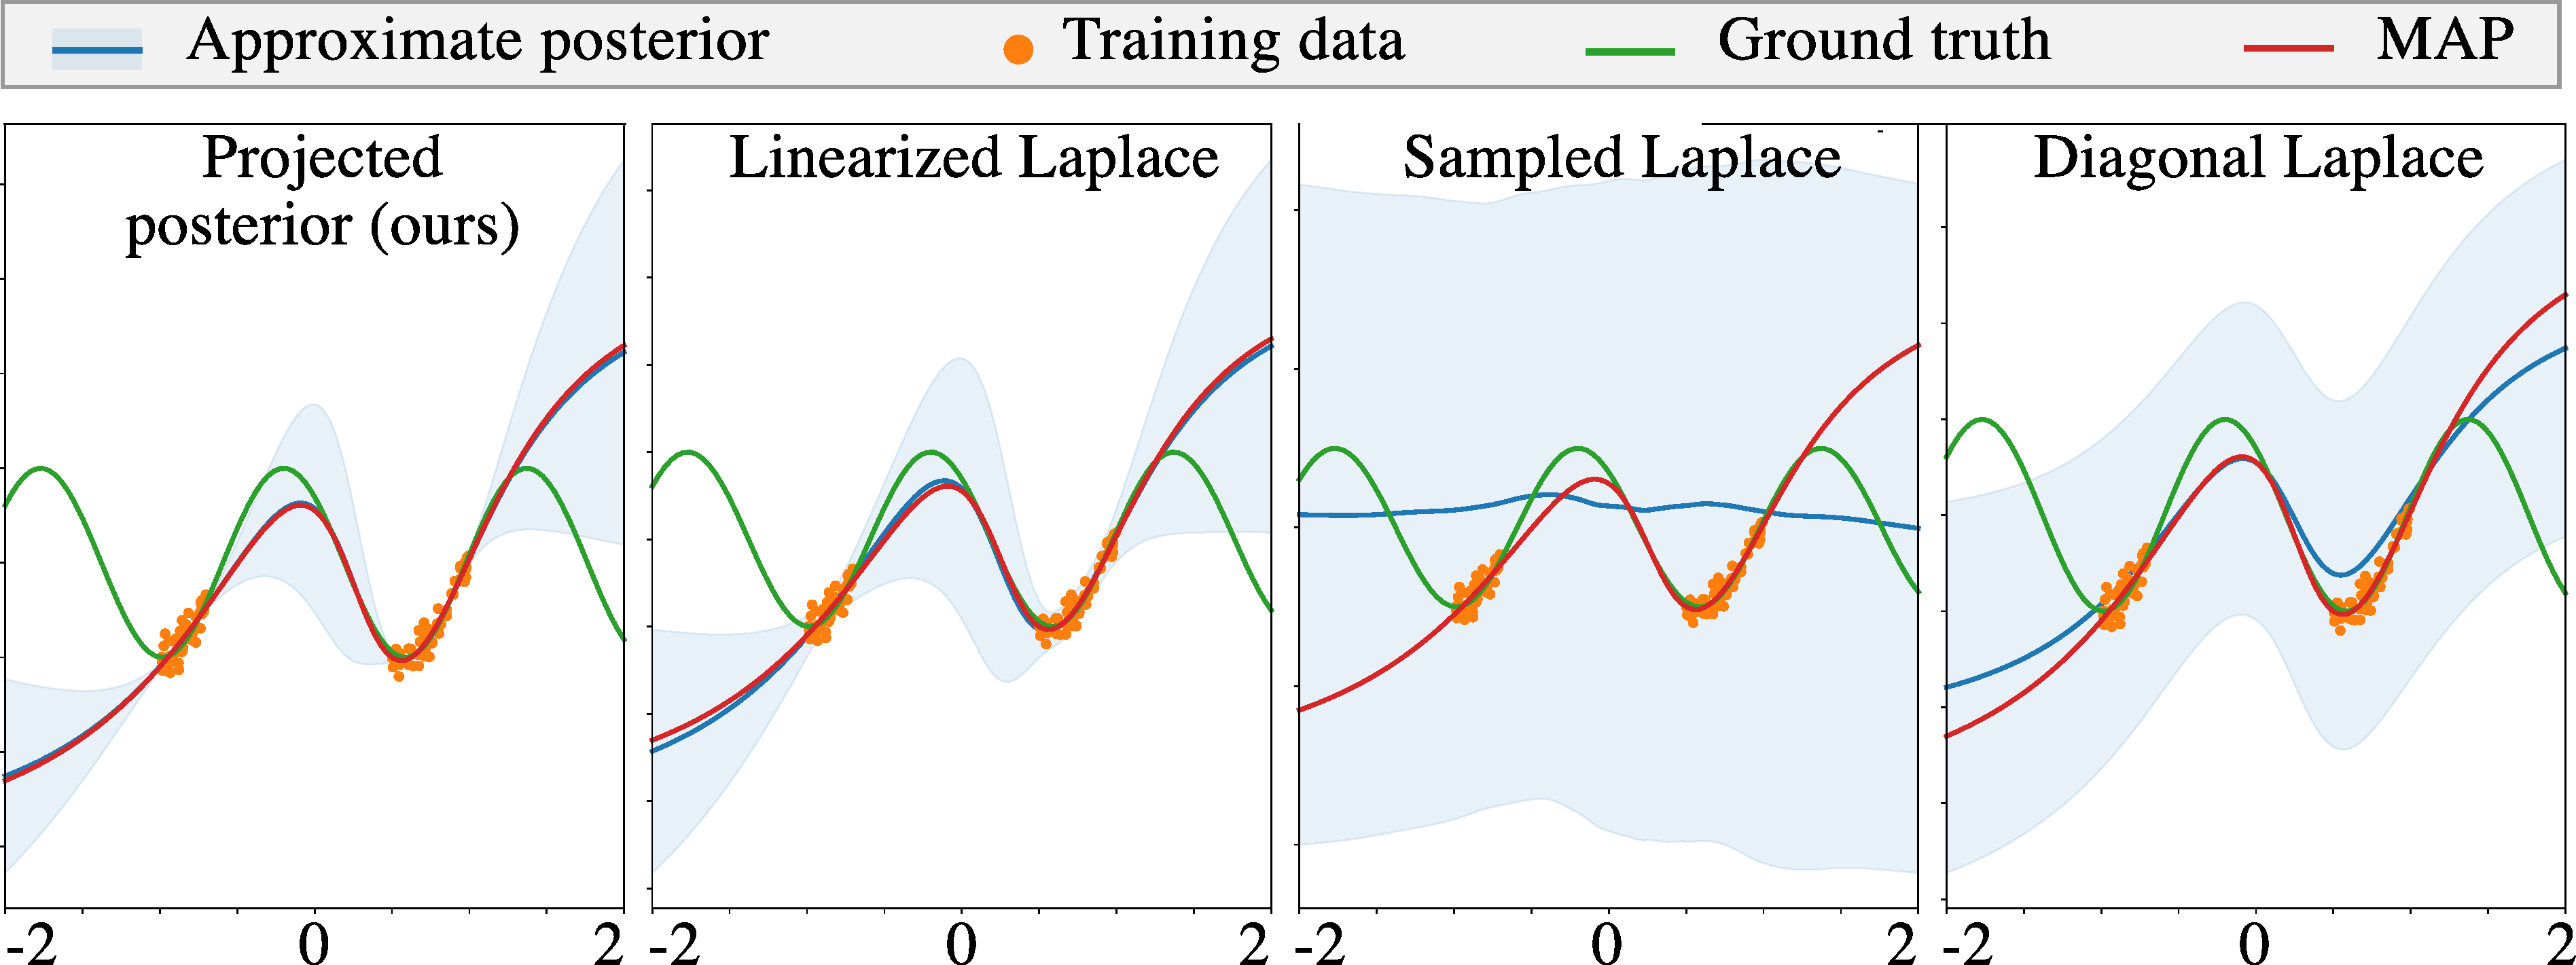
\includegraphics[width=\linewidth]{chapters/ch6_figures/in_between_uncertainty3.pdf}
  \vspace{-8mm}
  \caption{The sparse approximations of the posterior fail to capture in-between uncertainty, whereas fully correlated posteriors can capture it.}
  \label{fig:null_inbetween}
\end{figure}

\begin{mdframed}[backgroundcolor=myblue, linecolor=blue!75!black]
\textbf{Hypothesis:} The projected posterior captures in-between uncertainties better than sparsely correlated Laplace.
\end{mdframed}
We first assess different Laplace approximations in a toy regression task. \citet{foong2019between} shows that Bayesian neural networks with mean-field variational inference fail to capture in-between uncertainties.
We observe a similar issue with sparsely correlated Laplace approximations (Fig.~\ref{fig:null_inbetween}). In contrast, the projected posterior correlates all parameters, improving predictive uncertainty estimates for unseen regions. \emph{This illustrates that maintaining full parameter correlations is essential for accurate in-between uncertainties.}

\subsection{Predictive uncertainties on standard image classification}

\begin{mdframed}[backgroundcolor=myblue, linecolor=blue!75!black]
\textbf{Hypothesis:} The projected posterior provide competitive or superior predictive uncertainties across tasks, including in-distribution calibration, robustness to distribution shifts, and out-of-distribution detection.
\end{mdframed}

\paragraph{In-distribution performance (Table~\ref{tab:null_id}).}
We next consider standard image classification tasks. We train a LeNet \citep{lecun1989backpropagation} on MNIST and Fashion MNIST, and a ResNet \citep{he2016deep} on CIFAR-10 \citep{krizhevsky2009learning} and SVHN \citep{netzer2011reading}. Keeping the \MAP\ fixed we assess the predictive posterior of all methods using metrics such as confidence, accuracy, negative log-likelihood (NLL), Brier score \citep{VERIFICATIONOFFORECASTSEXPRESSEDINTERMSOFPROBABILITY}, expected calibration error (ECE), and maximum calibration error (MCE) \citep{naeini2015obtaining}.\looseness=-1

As shown in Table~\ref{tab:null_id}, the projected posterior matches \MAP\ in-distribution, as expected from Lemma~\ref{lm:null:zero_var_train}, with zero variance in-distribution and higher variance out-of-distribution. The loss-projected posterior improves calibration, which is discussed in Appendix B.

\begin{table*}
  \caption{In-distribution performance across methods trained on \textsc{mnist}, \textsc{fmnist} \smaller[0.80]{SVHN} and \smaller[0.80]{CIFAR-10}.}
  \label{tab:null_id}
  \setlength{\aboverulesep}{0pt}
  \setlength{\belowrulesep}{0pt}
  \setlength{\extrarowheight}{.75ex}
  \resizebox{\textwidth}{!}{
    \rotatebox[origin=c]{90}{MNIST~~~~~}\hspace{3mm}
    \begin{tabular}{lcccccc}
    \toprule \rowcolor{gray!30}
                            & Conf.~($\uparrow$)           & NLL~($\downarrow$)          & Acc.~($\uparrow$)           & Brier~($\downarrow$)        & ECE~($\downarrow$)        & MCE~($\downarrow$) \\
    \midrule
    MAP &
            0.981\small{±0.002} &
            0.080\small{±0.005} &
            \small{\first{0.977\small{±0.002}}} &
            1.775\small{±0.004} &
            0.787\small{±0.009} &
            0.895\small{±0.014} \\
    Projected posterior (ours)  &
            0.981\small{±0.002} &
            0.080\small{±0.005} &
            \small{\first{0.977\small{±0.002}}} &
            1.774\small{±0.004} &
            0.787\small{±0.009} &
            0.895\small{±0.014} \\
    Loss-projected posterior (ours) &
            0.813\small{±0.018} &
            1.225\small{±0.099} &
            0.949\small{±0.000} &
            \small{\first{1.532\small{±0.028}}} &
            \small{\first{0.666\small{±0.007}}} &
            0.894\small{±0.011} \\
    SWAG &
            \small{\first{0.982\small{±0.001}}} &
            \small{\first{0.064\small{±0.006}}} &
            0.982\small{±0.000} &
            1.776\small{±0.002} &
            0.788\small{±0.005} &
            0.906\small{±0.013} \\
    Last-Layer & 0.977\small{±0.002} & 0.090\small{±0.005} &
            0.975\small{±0.002} &
            1.768\small{±0.003} &
            0.784\small{±0.007} &
            \small{\first{0.887\small{±0.008}}} \\
    Diagonal &
            0.951\small{±0.008} &
            0.129\small{±0.016} &
            0.975\small{±0.001} &
            1.727\small{±0.012} &
            0.784\small{±0.008} &
            0.894\small{±0.015} \\
    \bottomrule
  \end{tabular} }
  \resizebox{\textwidth}{!}{
    \rotatebox[origin=c]{90}{FMNIST}\hspace{3mm}
    \begin{tabular}{lcccccc}
    MAP &
        \small{\first{0.938\small{±0.005}}} &
        0.325\small{±0.011} &
        0.897\small{±0.002} &
        1.713\small{±0.008} &
        0.732\small{±0.006} &
        0.901\small{±0.006} \\
    Projected posterior (ours) &
        0.937\small{±0.005} &
        \small{\first{0.325\small{±0.011}}} &
        0.897\small{±0.002} &
        1.713\small{±0.008} &
        0.732\small{±0.006} &
        0.902\small{±0.006} \\
    Loss-projected posterior (ours) &
        0.744\small{±0.031} &
        1.529\small{±0.371} &
        0.871\small{±0.006} &
        \small{\first{1.441\small{±0.041}}} &
        \small{\first{0.617\small{±0.025}}} &
        0.901\small{±0.013} \\
    SWAG &
        0.931\small{±0.006} &
        0.327\small{±0.001} &
        \small{\first{0.898\small{±0.001}}} &
        1.703\small{±0.008} &
        0.725\small{±0.003} &
        0.907\small{±0.003} \\
    Last Layer &
        0.931\small{±0.005} &
        0.339\small{±0.011} &
        0.896\small{±0.002} &
        1.703\small{±0.008} &
        0.727\small{±0.004} &
        0.902\small{±0.004} \\
    Diagonal &
        0.735\small{±0.024} &
        0.922\small{±0.051} &
        0.855\small{±0.000} &
        1.431\small{±0.033} &
        0.621\small{±0.021} &
        \small{\first{0.895\small{±0.021}}} \\
    \bottomrule
  \end{tabular} }
  \resizebox{\textwidth}{!}{
    \rotatebox[origin=c]{90}{SVHN}\hspace{3mm}
    \begin{tabular}{lcccccc}
    MAP &
            \small{\first{0.949\small{±0.004}}} &
            0.188\small{±0.004} &
            \small{\first{0.949\small{±0.002}}} &
            1.691\small{±0.004} &
            0.740\small{±0.012} &
            0.889\small{±0.004} \\
    Projected posterior (ours) &
            \small{\first{0.949\small{±0.004}}} &
            0.188\small{±0.004} &
            \small{\first{0.949\small{±0.002}}} &
            1.691\small{±0.004} &
            0.740\small{±0.012} &
            0.889\small{±0.007} \\
    Loss-projected posterior (ours) &
            0.948\small{±0.005} &
            0.191\small{±0.007} &
            \small{\first{0.949\small{±0.003}}} &
            1.685\small{±0.013} &
            \small{\first{0.734\small{±0.017}}} &
            0.880\small{±0.012} \\
    SWAG & 0.897±0.007 & 0.217±0.014 & 0.947±0.004 & \small{\first{1.606±0.010}} & 0.745±0.007 & \small{\first{0.874±0.003}} \\
    Last-Layer &
            0.943\small{±0.005} &
            0.197\small{±0.009} &
            0.946\small{±0.001} &
            1.681\small{±0.006} &
            0.740\small{±0.007} &
            0.899\small{±0.009} \\
    Diagonal &
            0.948\small{±0.003} &
            \small{\first{0.187\small{±0.005}}} &
            \small{\first{0.949\small{±0.002}}} &
            1.689\small{±0.003} &
            0.742\small{±0.011} &
            0.899\small{±0.000} \\
    \bottomrule
  \end{tabular} }
  \resizebox{\textwidth}{!}{
    \rotatebox[origin=c]{90}{CIFAR-10}\hspace{3mm}
    \begin{tabular}{lcccccc}
    MAP &
            \small{\first{0.952\small{±0.002}}} &
            0.422\small{±0{.011}} &
            \small{\first{0.894\small{±0.002}}} &
            1.698\small{±0.038} &
            0.703\small{±0.013} &
            0.878\small{±0.009} \\
    Projected posterior (ours) &
            \small{\first{0.952\small{±0.001}}} &
            0.422\small{±0{.011}} &
            \small{\first{0.894\small{±0.002}}} &
            1.698\small{±0.038} &
            0.703\small{±0.013} &
            0.878\small{±0.002} \\
    Loss-projected posterior (ours) &
            0.701\small{±0.013} &
            2.643\small{±0.205} &
            0.855\small{±0.002} &
            \small{\first{1.387\small{±0.018}}} &
            \small{\first{0.559\small{±0.006}}} &
            \small{\first{0.802\small{±0.005}}} \\
    SWAG &
            0.914\small{±0.035} &
            0.445\small{±0.063} &
            0.865\small{±0.029} &
            1.670\small{±0.049} &
            0.694\small{±0.018} &
            0.881\small{±0.005} \\
    Last-Layer &
            0.944\small{±0.001} &
            \small{\first{0.406\small{±0.005}}} &
            \small{\first{0.894\small{±0.001}}} &
            1.712\small{±0.001} &
            0.704\small{±0.000} &
            0.880\small{±0.007} \\
    Diagonal &
            0.934\small{±0.028} &
            0.465\small{±0.069} &
            0.872\small{±0.032} &
            1.698\small{±0.038} &
            0.703\small{±0.013} &
            0.873\small{±0.005} \\
    \bottomrule
  \end{tabular} }
\end{table*}

\begin{table*}
  \caption{Out-of-distribution \textsc{auroc}~($\uparrow$) performance for \textsc{mnist}, \textsc{fmnist}, \smaller[0.80]{SVHN} and \smaller[0.80]{CIFAR-10}.}
  \label{tab:null_ood}
  \setlength{\aboverulesep}{0pt}
  \setlength{\belowrulesep}{0pt}
  \setlength{\extrarowheight}{.75ex}
  \resizebox{\textwidth}{!}{
    \begin{tabular}{lcccccccccc}
    \toprule
    \rowcolor{gray!30} Trained on & \multicolumn{3}{c}{\rule[0.9mm]{20mm}{0.1mm} \textsc{mnist} \rule[0.9mm]{20mm}{0.1mm}} & \multicolumn{3}{c}{\rule[0.9mm]{20mm}{0.1mm} \textsc{fmnist} \rule[0.9mm]{20mm}{0.1mm}} & \multicolumn{2}{c}{\rule[0.9mm]{12mm}{0.1mm} \smaller[0.80]{CIFAR-10} \rule[0.9mm]{12mm}{0.1mm}} &
    \multicolumn{2}{c}{\rule[0.9mm]{12mm}{0.1mm} \smaller[0.80]{SVHN} \rule[0.9mm]{12mm}{0.1mm}}
    \\
    \rowcolor{gray!30} Tested on & \textsc{fmnist} & \textsc{emnist} & \textsc{kmnist} & \textsc{mnist} & \textsc{emnist} & \textsc{kmnist} & \textsc{svhn} & \smaller[0.80]{CIFAR-100} & \smaller[0.80]{CIFAR-10} & \smaller[0.80]{CIFAR-100} \\
    \midrule
    MAP & 0.924±0.015 & 0.888±0.010 & 0.846±0.019 & 0.714±0.001 & 0.788±0.016 & 0.664±0.012 & 0.874±0.002 & 0.816±0.026 &
    0.960±0.007 & 0.954±0.008\\
    Proj.\@ (ours) & \first{0.926±0.013} & 0.904±0.004 & \first{0.862±0.011} & 0.861±0.029 & 0.844±0.032 & 0.867±0.012 & \first{0.881±0.002} & \first{0.836±0.004} &
    0.960±0.002 & 0.957±0.001\\
    Loss-proj.\@ (ours) & 0.899±0.011 & 0.893±0.006 & 0.856±0.002 & \first{0.914±0.035} & \first{0.928±0.007} & \first{0.907±0.026} & 0.863±0.008 & 0.800±0.013 &
    \first{0.966±0.009} & \first{0.960±0.006}\\
    SWAG & 0.917±0.024 & \first{0.916±0.010}  & 0.861±0.032 &
            0.685±0.014 & 0.751±0.032 & 0.655±0.015 & 0.798±0.040 & 0.782±0.042 &
            0.777±0.029 & 0.787±0.027\\
    Last-Layer & 0.793±0.215 & 0.782±0.182 & 0.759±0.166 &
                   0.768±0.001 & 0.824±0.016 & 0.699±0.020 & 0.811±0.024 & 0.801±0.026 &
                   0.914±0.005 & 0.908±0.005\\
    Diagonal & 0.772±0.218 & 0.768±0.191 & 0.745±0.174 &
                0.726±0.028 & 0.725±0.034 & 0.683±0.013 & 0.836±0.022 & 0.806±0.027 &
                0.917±0.005 & 0.916±0.004\\
    \bottomrule
  \end{tabular} }
\end{table*}

\begin{table*}
  \caption{In- and out-of-distribution metrics for SWIN transformer trained on ImageNet and tested on \textsc{places365}.}
  \label{tab:null_imagenet}
  \setlength{\aboverulesep}{0pt}
  \setlength{\belowrulesep}{0pt}
  \setlength{\extrarowheight}{.75ex}
  \resizebox{0.7\textwidth}{!}{
    \begin{tabular}{lccccccc}
    \toprule
    \rowcolor{gray!30}
    & Conf.~($\uparrow$)           & NLL~($\downarrow$)      & Acc.~($\uparrow$)           & Brier~($\downarrow$)
    & ECE~($\downarrow$)        & MCE~($\downarrow$)
    & AUROC ~($\uparrow$)             \\
    \midrule
    \textsc{map} & \first{0.626} & \first{1.358} & \first{0.726} & 0.407 & 0.136 & 0.583 & 0.751 \\
    Loss-projected posterior & 0.618 & 1.427 & 0.716 & \first{0.394} & \first{0.107} & \first{0.259} & \first{0.756} \\
    \bottomrule
  \end{tabular} }
\end{table*}

\begin{figure*}
  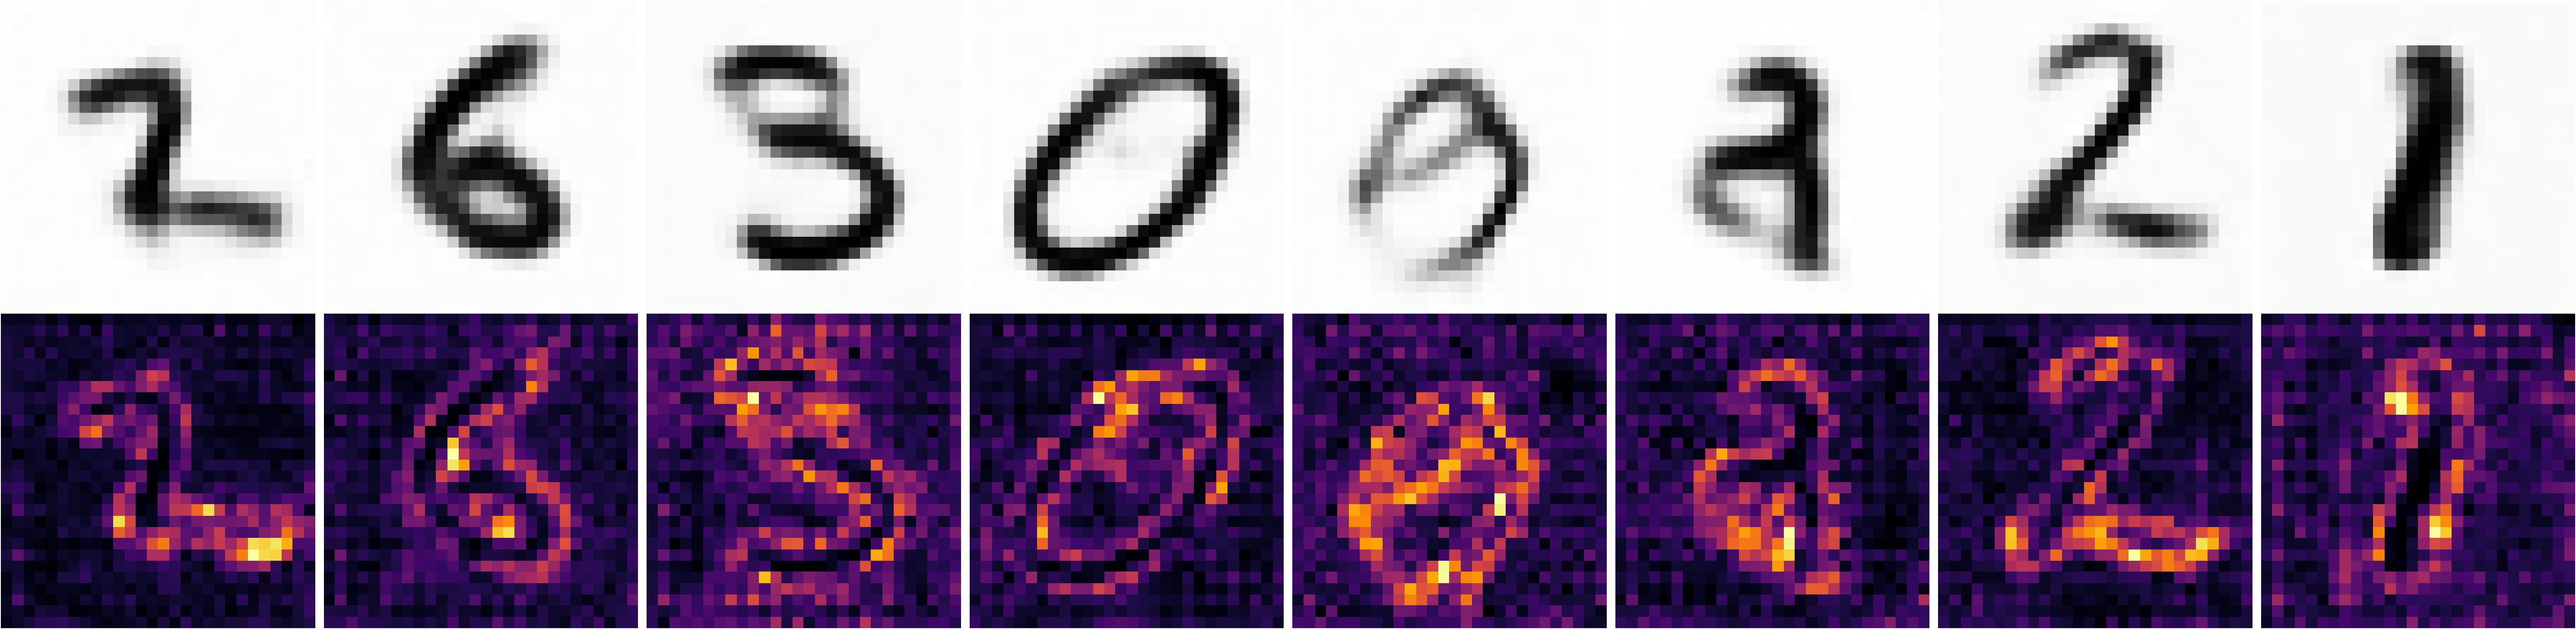
\includegraphics[width=0.49\linewidth]{chapters/ch6_figures/MNIST_std_gen_1.pdf}
  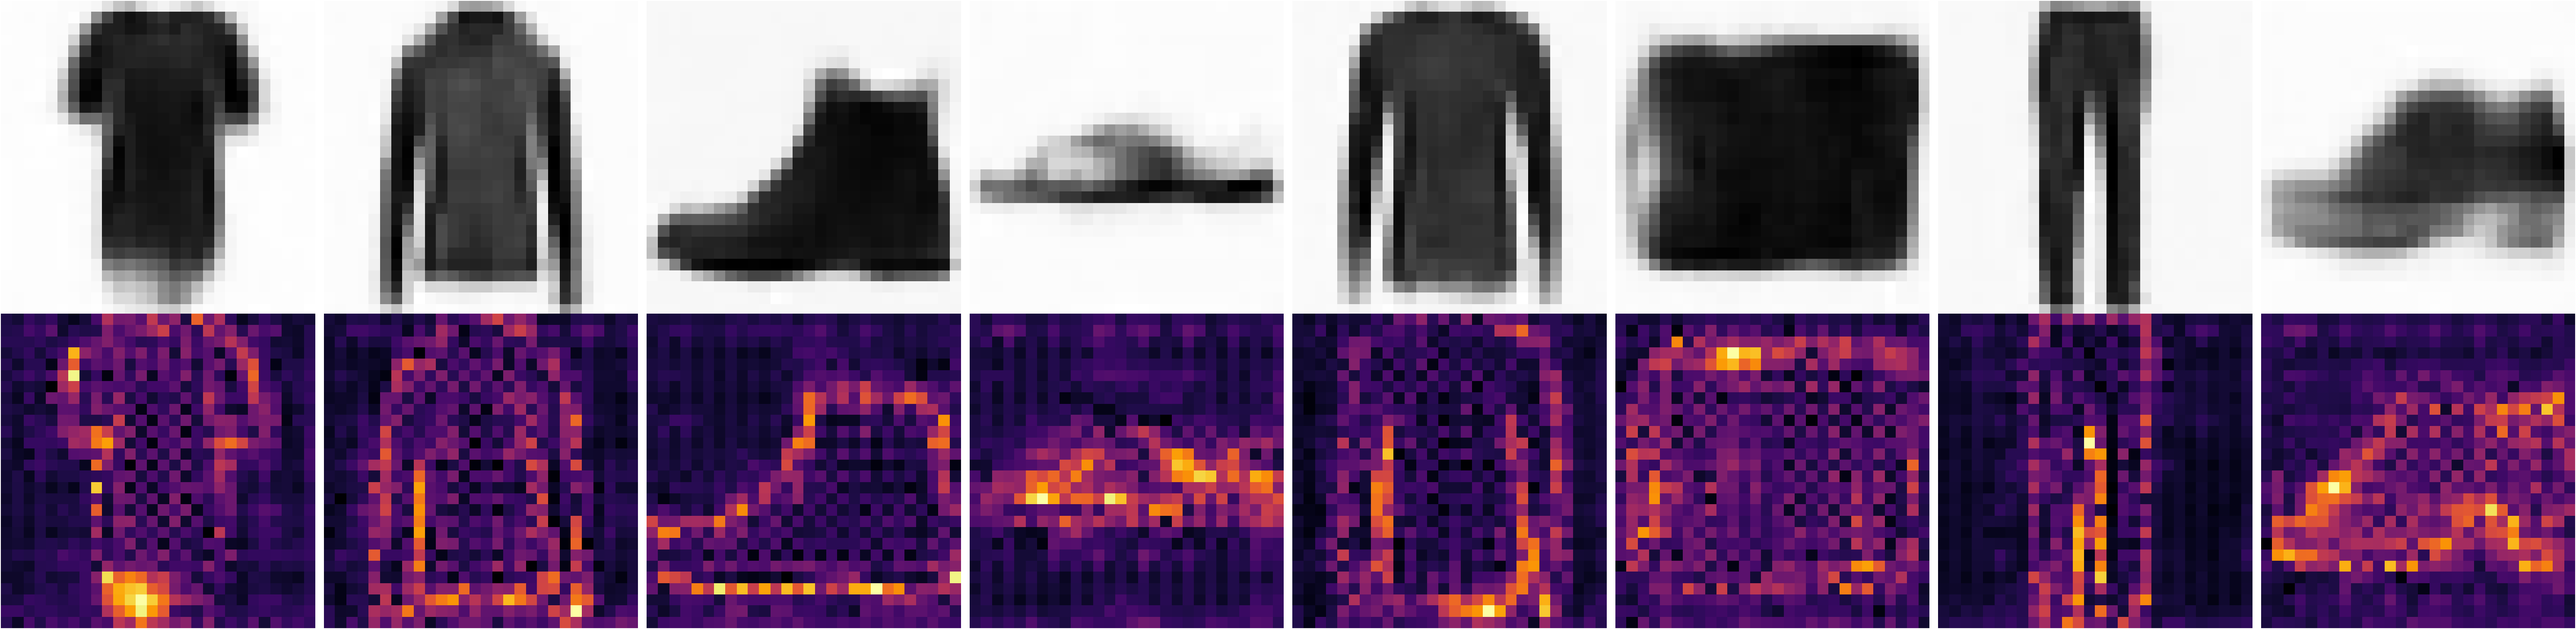
\includegraphics[width=0.49\linewidth]{chapters/ch6_figures/FMNIST_std_gen_1.pdf}
  \vspace{-4mm}
  \caption{\textbf{Variational autoencoder reconstructions and corresponding uncertainty estimates.} \emph{Left:} mean reconstructions of MNIST and Fashion MNIST images sampled from the latent space. \emph{Right:} pixel-wise uncertainty estimates generated by sampling decoder parameters from the loss-projected posterior, highlighting key semantic features such as edges and contours. This demonstrates that the loss-projected posterior scales to high-dimensional generative models.}
  \label{fig:null_vae_variance}
\end{figure*}

\paragraph{Distribution shift (Fig.~\ref{fig:null_shift_plots}).}
To assess robustness under distribution shifts, we evaluate predictive uncertainties using \textsc{rotated-mnist}, \textsc{rotated-fmnist}, and \textsc{corrupted cifar} (with fog and Gaussian blur). The loss-projected posterior maintains low, stable calibration error with increasing shift intensity, while the projected posterior retains high accuracy (Fig.~\ref{fig:null_shift_plots}).

\begin{figure}[t]
  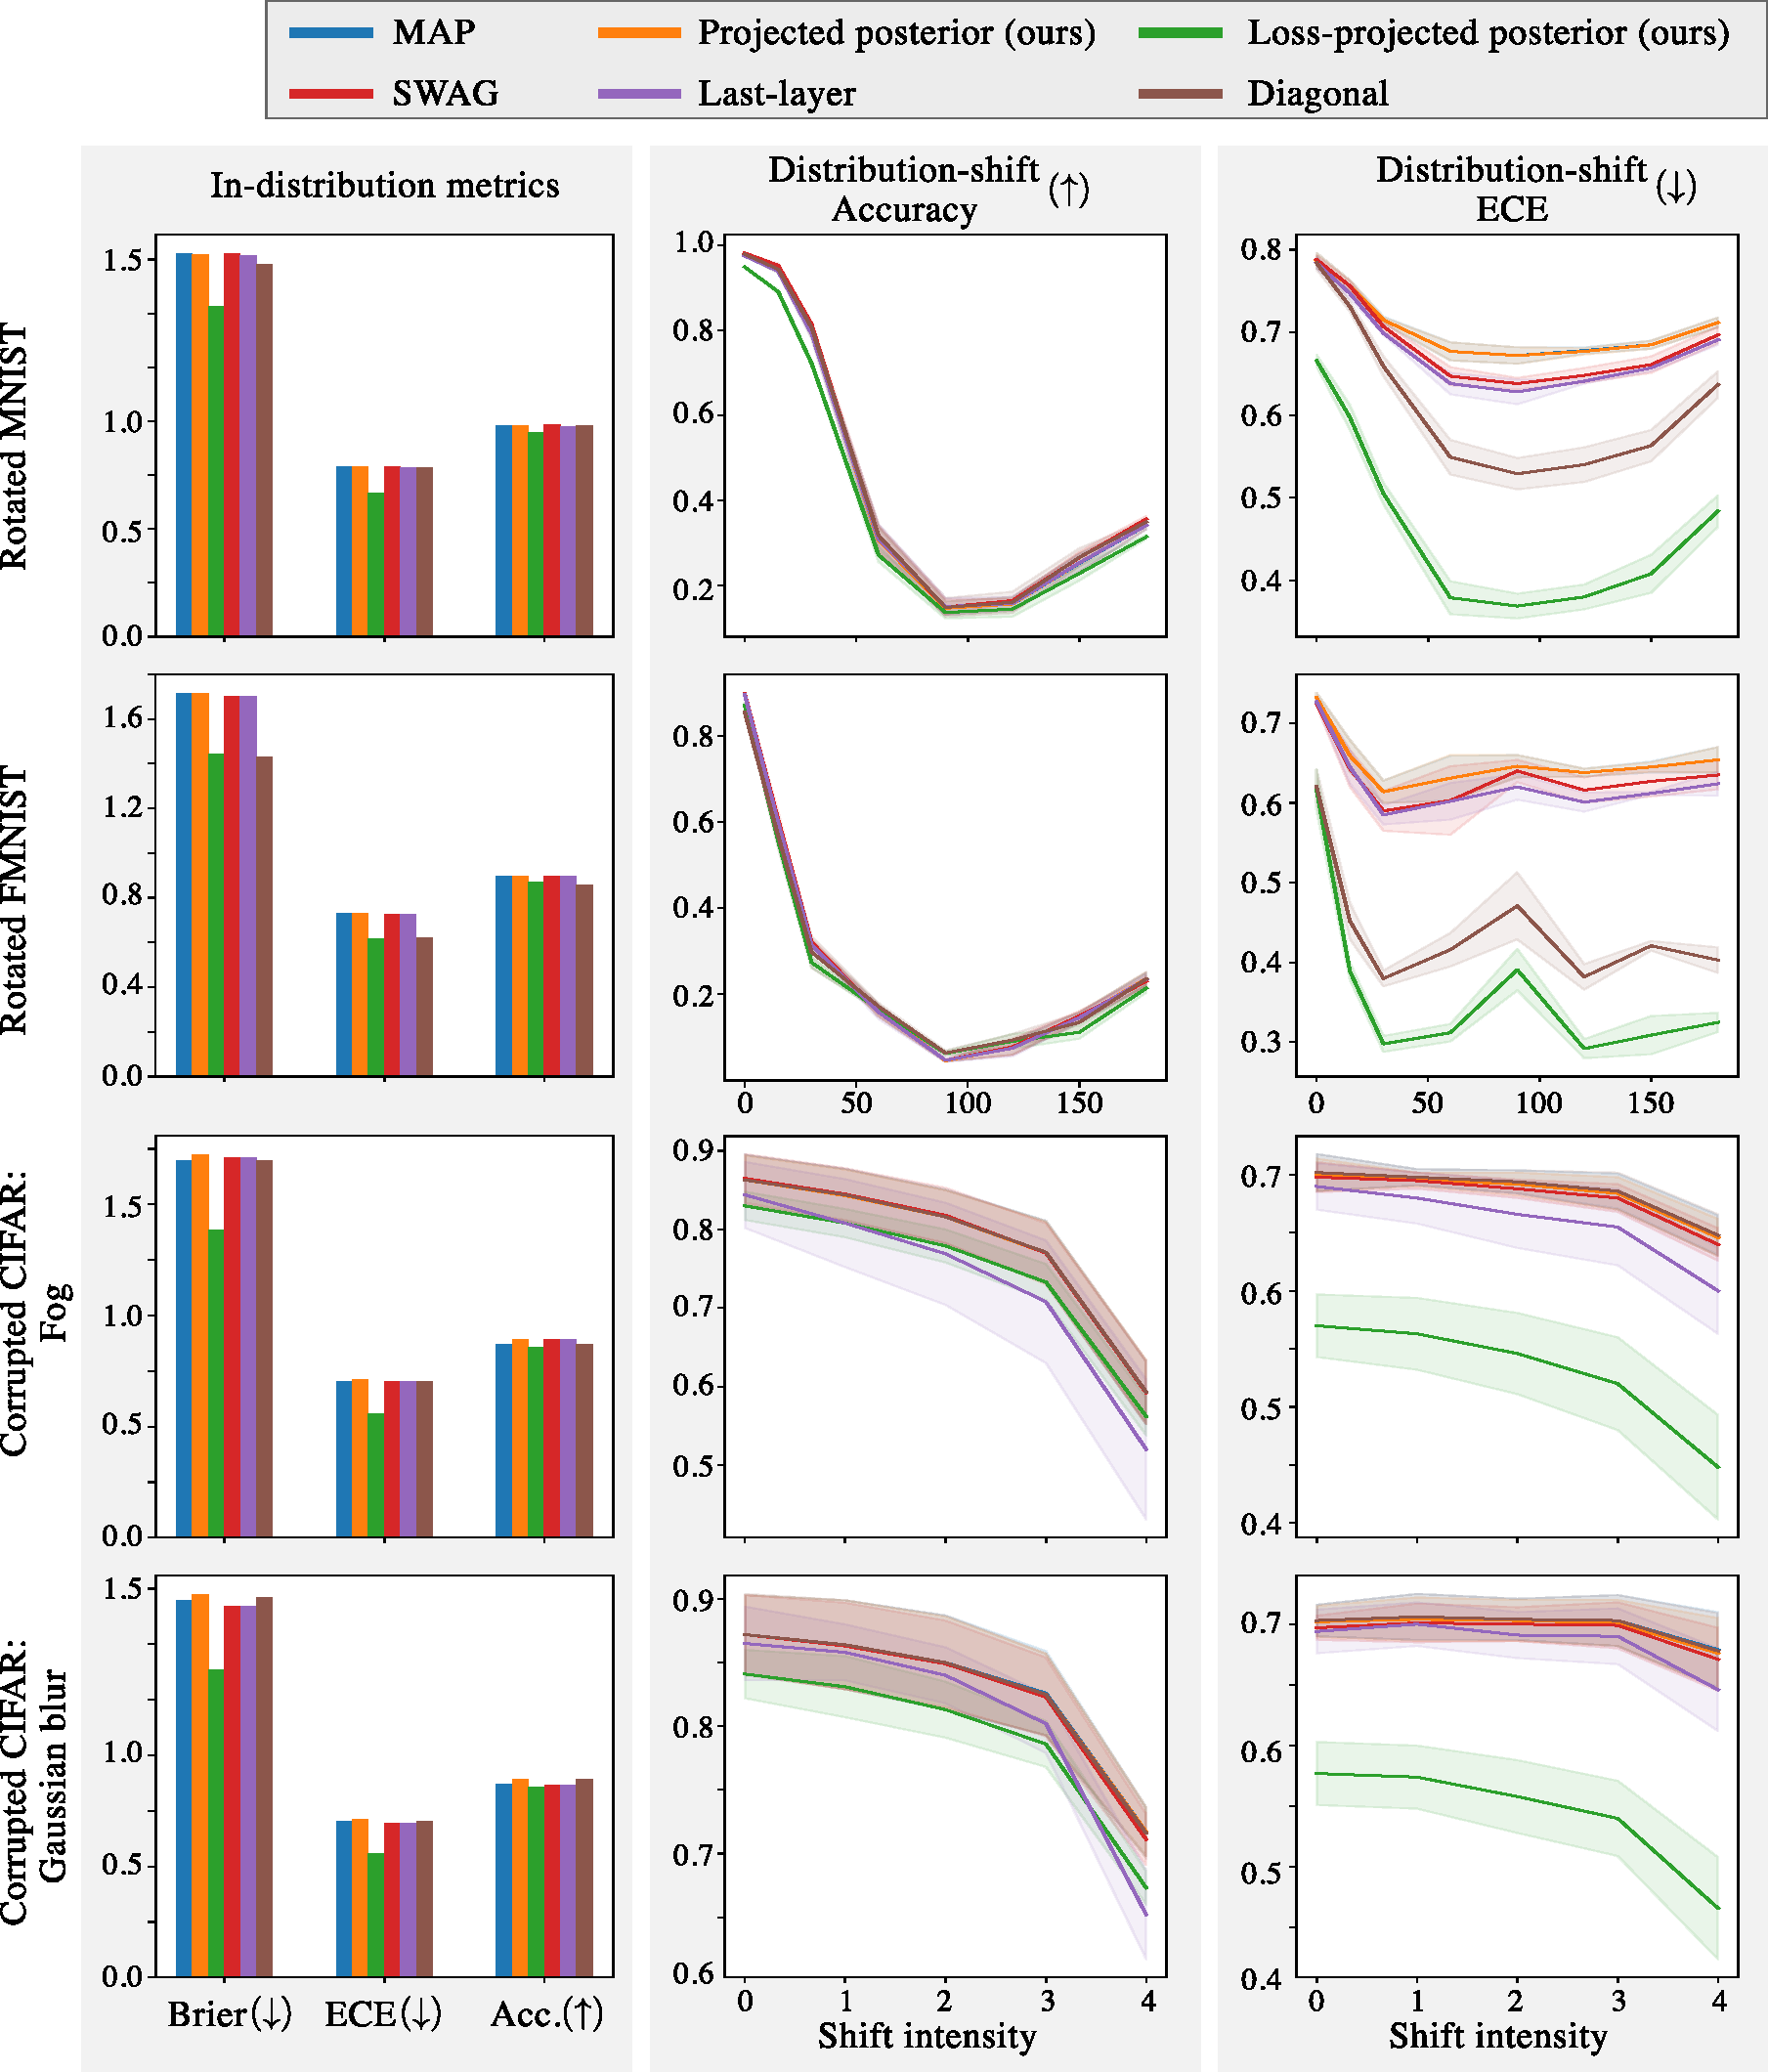
\includegraphics[width=\linewidth]{chapters/ch6_figures/corrupted3.pdf}
  \vspace{-8mm}
  \caption{Model calibration and fit on in-distribution test data (left) and under distribution shift (middle, right) where we plot shift intensities against accuracy and expected calibration error (\textsc{ece}), respectively.}
  \label{fig:null_shift_plots}
\end{figure}

\paragraph{Out-of-distribution detection (Table~\ref{tab:null_ood}).}
For out-of-distribution (\textsc{ood}) detection, we use the maximum variance of logits across output dimensions as an \textsc{ood} score for all Bayesian posteriors, while the \MAP\ baseline employs maximum softmax, which is a strong baseline. Lemma~\ref{lm:null:zero_var_train} dictates that the in-distribution variance of the projected posterior is zero, providing a strong \textsc{ood} detection signal. Table~\ref{tab:null_ood} supports the theory, showing that the projected posterior achieves superior \textsc{auroc} scores across various \textsc{ood} tasks over baselines.

\subsection{ImageNet and CelebA vision transformer}

\begin{mdframed}[backgroundcolor=myblue, linecolor=blue!75!black]
\textbf{Hypothesis:} The projected posterior scales effectively to large models and datasets, such as SWIN transformers trained on ImageNet and CelebA.
\end{mdframed}

We assess the scalability of our approach by sampling from the loss-projected posterior of a SWIN transformer \citep{liu2021swin} pre-trained on the ImageNet-1K dataset \citep{deng2009imagenet, russakovsky2015imagenet}, which includes about 1 million images of size $224\times224\times3$ with 1000 output classes. Table~\ref{tab:null_imagenet} shows marginal improvement in-distribution calibration over \MAP\ alongside improved out-of-distribution detection on \textsc{places365} \citep{zhou2017places}. \emph{The main point is that our method scales gracefully to large models and datasets due to linear complexity.}

We further consider a 4M-parameter Visual Attention network (\textsc{VAN}) \citep{guo2023visual}. We train on \textsc{CelebA} \citep{liu2015faceattributes} holding out three classes. \cref{tab:null_celeba} reports \textsc{auroc} scores to measure the ability to detect the three held-out classes and \textsc{Food101} \citep{bossard2014food} as out-of-distribution. Both our method and baselines have a limited memory budget of $300P$ numbers. \LLA\ and local ensemble are implemented using Lanczos and we also include our projected score computed with Lanczos as a reference.
The projected posterior outperforms the baselines on the three most challenging settings and is only second to \textsc{scod} in the last. The loss-projected posterior shows a minor drop in performance.

\begin{table}[t]
    \vspace{-3mm}
    \caption{\textsc{auroc} (3 seeds) for a \textsc{VAN} trained on \textsc{CelebA}. Details are in the appendix.}
    \label{tab:null_celeba}
    \setlength{\aboverulesep}{0pt}
    \setlength{\belowrulesep}{0pt}
    \setlength{\extrarowheight}{.75ex}
    \resizebox{\linewidth}{!}{
    \begin{tabular}{lcccc}
    \toprule
    \rowcolor{gray!30}
        & Food101 & Bald only & Eyeglasses only & Mustache only \\ \midrule
    Max logit & 0.959$\pm$0.008  & 0.32$\pm$0.00  & 0.57$\pm$0.01  & 0.40$\pm$0.03  \\
    Deep ensemble & 0.957  & 0.71  & 0.74  & 0.61  \\
    Proj.\@ (ours) & 0.958$\pm$0.004  & \first{0.81$\pm$0.03}  & \first{0.75$\pm$0.01}  & \first{0.66$\pm$0.01}  \\
    Loss-proj.\@ (ours) & 0.947$\pm$0.007  & 0.76$\pm$0.03  & 0.72$\pm$0.01  & 0.62$\pm$0.01  \\
    Proj-Lanczos & 0.954$\pm$0.004  & 0.80$\pm$0.03  & 0.74$\pm$0.01  & 0.64$\pm$0.01  \\
    Local ensemble & 0.951$\pm$0.003  & 0.79$\pm$0.04  & 0.73$\pm$0.01  & 0.63$\pm$0.01  \\
    LLA & 0.954$\pm$0.00  & 0.80$\pm$0.03  & 0.74$\pm$0.01  & 0.64$\pm$0.01  \\
    LLA-diag & 0.797$\pm$0.021  & 0.54$\pm$0.03  & 0.57$\pm$0.02  & 0.45$\pm$0.03  \\
    SCOD & \first{0.964$\pm$0.000}  & 0.79$\pm$0.03  & 0.73$\pm$0.01  & 0.64$\pm$0.01  \\
    SWAG & 0.740$\pm$0.021  & 0.70$\pm$0.08  & 0.52$\pm$0.04  & 0.49$\pm$0.04 \\
    SLU & 0.953$\pm$0.003  & 0.80$\pm$0.03  & 0.74$\pm$0.01  & 0.64$\pm$0.01 \\
    \bottomrule
    \end{tabular}
    }
\end{table}

\subsection{Generative models}

\begin{mdframed}[backgroundcolor=myblue, linecolor=blue!75!black]
\textbf{Hypothesis:} The loss-projected posterior scales to generative models with large output dimensions.
\end{mdframed}

We evaluate the loss-projected posterior on variational autoencoders \citep{kingma2013auto} trained on \textsc{MNIST} and \textsc{Fashion MNIST}, showcasing its flexibility with high-dimensional outputs and diverse tasks. After training, we sample decoder parameters to generate images from latent space samples. Fig.~\ref{fig:null_vae_variance} shows that the sampled decoders produce diverse reconstructions with pixel-wise uncertainty estimates that capture meaningful features.\looseness=-1

\emph{This experiment highlights that our approach scales to generative models while preserving essential predictive uncertainties.} Its adaptability beyond classification makes it a robust tool for diverse tasks.